\chapter{Test Datasets}
For data synthesis, good and realistic data is necessary. For this project, many test datasets were used in order to implement, test and evaluate the tool. In this appendix, you will find the most important dataset that was used to develop and test this tool with.
\section{Tennis ATP}
\label{sec:tennis_atp_dataset}
Tennis ATP is a dataset consisting of realistic data of the Tennis ATP (Association of Tennis Professionals). It includes rankings of players, data about the players themselves, data about the matches played between those players etc. \\
\newline
The repository for the complete data set can be found here: \url{https://github.com/JeffSackmann/tennis\_atp}. The complete dataset found in the repository however,  is not entirely used in this tool, only some chunks of it. The data set chunks used for this tool have been chosen and provided by my advisor: Prof. Stefan Keller.\\
\begin{figure}[H]
	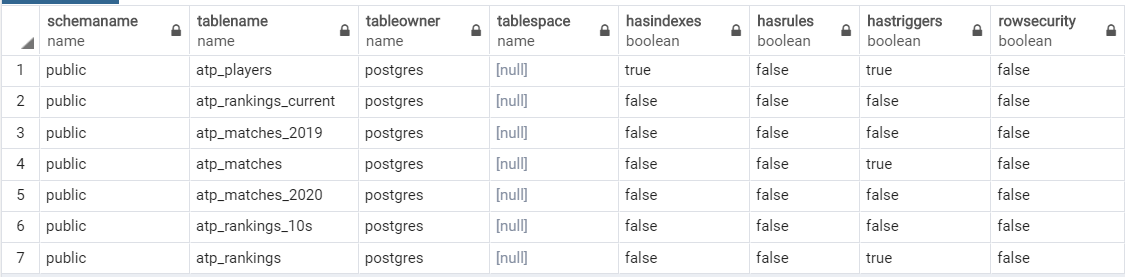
\includegraphics[width=\linewidth]{./Figures/Appendices/tennis_atp_schema.png}
	\caption{Tennis ATP database schema}
\end{figure}
\newpage
The columns of the tables are realistic and make sense. They also make sense in the context of synthesizing them.
\begin{figure}[H]
	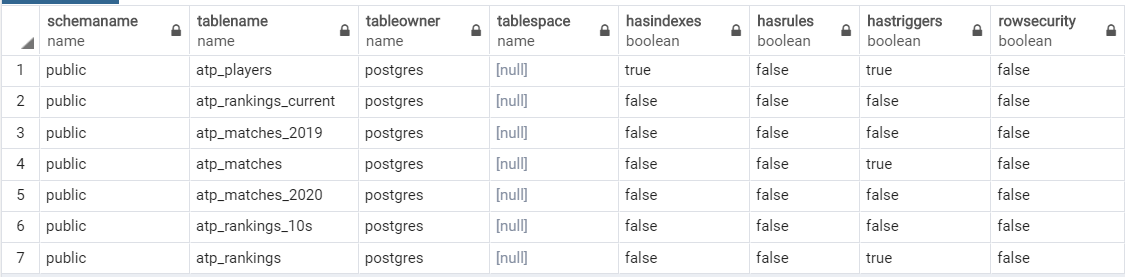
\includegraphics[width=\linewidth]{./Figures/Appendices/tennis_atp_schema.png}
	\caption{Tennis ATP database schema}
\end{figure}
\begin{figure}[H]
	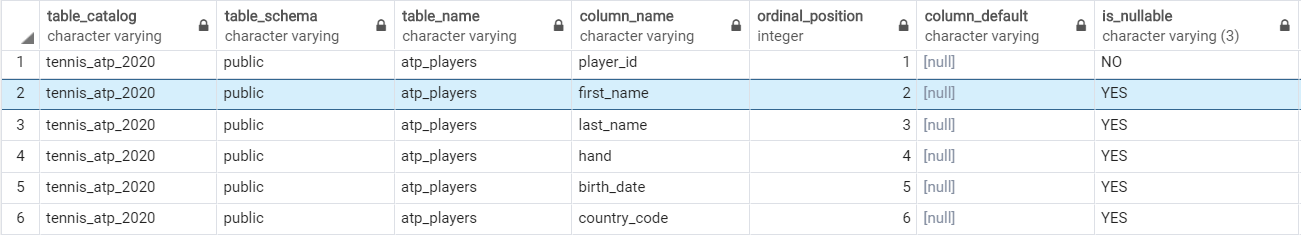
\includegraphics[width=\linewidth]{./Figures/Appendices/tennis_atp_players_schema.png}
	\caption{Tennis ATP "atp\_players" table schema}
\end{figure}
\begin{figure}[H]
	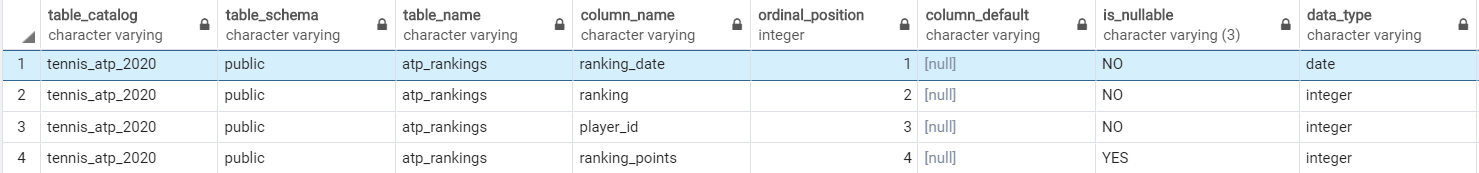
\includegraphics[width=\linewidth]{./Figures/Appendices/tennis_atp_rankings_schema.png}
	\caption{Tennis ATP "atp\_rankings" table schema}
\end{figure}
\begin{figure}[H]
	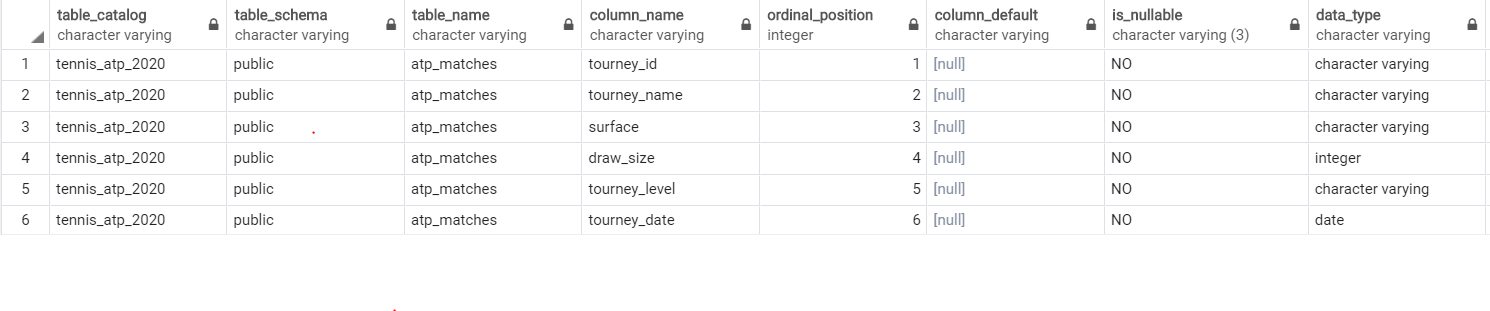
\includegraphics[width=\linewidth]{./Figures/Appendices/tennis_atp_matches_schema_1.png}
	\caption{Some information from the Tennis ATP "atp\_matches" table schema \#1}
\end{figure}
\begin{figure}[H]
	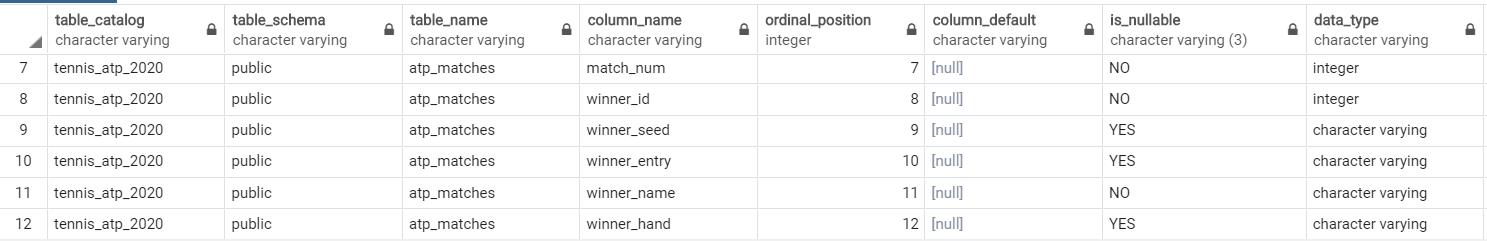
\includegraphics[width=\linewidth]{./Figures/Appendices/tennis_atp_matches_schema_2.png}
	\caption{Some information from the Tennis ATP "atp\_matches" table schema \#2}
\end{figure}